%% This manuscript uses the AASTeX v6.2 LaTeX 2e macros
%%
%% AASTeX is now based on Alexey Vikhlinin's emulateapj.cls
%% (Copyright 2000-2015).  See the classfile for details.

%% AASTeX requires revtex4-1.cls (http://publish.aps.org/revtex4/) and
%% other external packages (latexsym, graphicx, amssymb, longtable, and epsf).
%% All of these external packages should already be present in the modern TeX
%% distributions.  If not they can also be obtained at www.ctan.org.

%% The first piece of markup in an AASTeX v6.x document is the \documentclass
%% command. LaTeX will ignore any data that comes before this command. The
%% documentclass can take an optional argument to modify the output style.
%% The command below calls the preprint style  which will produce a tightly
%% typeset, one-column, single-spaced document.  It is the default and thus
%% does not need to be explicitly stated.
%%
%%
%% using aastex version 6.2
\documentclass{aastex62}

%% The default is a single spaced, 10 point font, single spaced article.
%% There are 5 other style options available via an optional argument. They
%% can be envoked like this:
%%
%% \documentclass[argument]{aastex62}
%%
%% where the layout options are:
%%
%%  twocolumn   : two text columns, 10 point font, single spaced article.
%%                This is the most compact and represent the final published
%%                derived PDF copy of the accepted manuscript from the publisher
%%  manuscript  : one text column, 12 point font, double spaced article.
%%  preprint    : one text column, 12 point font, single spaced article.
%%  preprint2   : two text columns, 12 point font, single spaced article.
%%  modern      : a stylish, single text column, 12 point font, article with
%% 		  wider left and right margins. This uses the Daniel
%% 		  Foreman-Mackey and David Hogg design.
%%  RNAAS       : Preferred style for Research Notes which are by design
%%                lacking an abstract and brief. DO NOT use \begin{abstract}
%%                and \end{abstract} with this style.
%%
%% Note that you can submit to the AAS Journals in any of these 6 styles.
%%
%% There are other optional arguments one can envoke to allow other stylistic
%% actions. The available options are:
%%
%%  astrosymb    : Loads Astrosymb font and define \astrocommands.
%%  tighten      : Makes baselineskip slightly smaller, only works with
%%                 the twocolumn substyle.
%%  times        : uses times font instead of the default
%%  linenumbers  : turn on lineno package.
%%  trackchanges : required to see the revision mark up and print its output
%%  longauthor   : Do not use the more compressed footnote style (default) for
%%                 the author/collaboration/affiliations. Instead print all
%%                 affiliation information after each name. Creates a much
%%                 long author list but may be desirable for short author papers
%%
%% these can be used in any combination, e.g.
%%
%% \documentclass[twocolumn,linenumbers,trackchanges]{aastex62}
%%
%% AASTeX v6.* now includes \hyperref support. While we have built in specific
%% defaults into the classfile you can manually override them with the
%% \hypersetup command. For example,
%%
%%\hypersetup{linkcolor=red,citecolor=green,filecolor=cyan,urlcolor=magenta}
%%
%% will change the color of the internal links to red, the links to the
%% bibliography to green, the file links to cyan, and the external links to
%% magenta. Additional information on \hyperref options can be found here:
%% https://www.tug.org/applications/hyperref/manual.html#x1-40003
%%
%% If you want to create your own macros, you can do so
%% using \newcommand. Your macros should appear before
%% the \begin{document} command.
%%
\newcommand{\vdag}{(v)^\dagger}
\newcommand\aastex{AAS\TeX}
\newcommand\latex{La\TeX}

% for non-stacked fractions
\newcommand{\sfrac}[2]{\mathchoice
  {\kern0em\raise.5ex\hbox{\the\scriptfont0 #1}\kern-.15em/
   \kern-.15em\lower.25ex\hbox{\the\scriptfont0 #2}}
  {\kern0em\raise.5ex\hbox{\the\scriptfont0 #1}\kern-.15em/
   \kern-.15em\lower.25ex\hbox{\the\scriptfont0 #2}}
  {\kern0em\raise.5ex\hbox{\the\scriptscriptfont0 #1}\kern-.2em/
   \kern-.15em\lower.25ex\hbox{\the\scriptscriptfont0 #2}}
  {#1\!/#2}}

\newcommand{\myhalf}{\sfrac{1}{2}}
\newcommand{\thalf}{\sfrac{3}{2}}

\newcommand{\eb}{{\bf{e}}}
\newcommand{\Ub}{{\bf{U}}}
\newcommand{\Ubt}{\widetilde{\Ub}}
\newcommand{\Vb}{{\bf{V}}}
\newcommand{\xb}{{\bf{x}}}

\newcommand{\dr}{\Delta r}
\newcommand{\dt}{\Delta t}

\newcommand{\etarho}{\eta_\rho}
\newcommand{\gammaonebar}{\overline{\Gamma}_1}
\newcommand{\Hnuc}{H_{\rm nuc}}
\newcommand{\omegadot}{\dot\omega}
\newcommand{\pred}{{\rm pred}}
\newcommand{\Sbar}{\overline{S}}

\newcommand{\inp}{\mathrm{in}}
\newcommand{\outp}{\mathrm{out}}
\newcommand{\nph}{{n+\myhalf}}
\newcommand{\nmh}{{n-\myhalf}}
\newcommand{\ow}{\overline{w_0}}
\newcommand{\dw}{\delta w_0}
\newcommand{\uadvone}{\Ub^{\mathrm{ADV},\star}}
\newcommand{\uadvonedag}{\Ub^{\mathrm{ADV},\dagger,\star}}
\newcommand{\uadvtwo}{\Ub^{\mathrm{ADV}}}
\newcommand{\uadvtwodag}{\Ub^{\mathrm{ADV},\dagger}}
\newcommand{\gcc}{\mathrm{g~cm^{-3} }}

% for the red MarginPars
\usepackage{color}
% make the MarginPars look pretty
\setlength{\marginparwidth}{0.5in}
\newcommand{\MarginPar}[1]{\marginpar{\vskip-\baselineskip\raggedright\tiny\sffamily
\hrule\smallskip{\color{red}#1}\par\smallskip\hrule}}

\usepackage{url}

\usepackage{mathtools}

\usepackage{multirow}

%% Reintroduced the \received and \accepted commands from AASTeX v5.2
\received{XXX X, XXXX}
\revised{XXX X, XXXX}
\accepted{XXX X, XXXX}
%% Command to document which AAS Journal the manuscript was submitted to.
%% Adds "Submitted to " the arguement.
\submitjournal{ApJ}

%% Mark up commands to limit the number of authors on the front page.
%% Note that in AASTeX v6.2 a \collaboration call (see below) counts as
%% an author in this case.
%
%\AuthorCollaborationLimit=3
%
%% Will only show Schwarz, Muench and "the AAS Journals Data Scientist
%% collaboration" on the front page of this example manuscript.
%%
%% Note that all of the author will be shown in the published article.
%% This feature is meant to be used prior to acceptance to make the
%% front end of a long author article more manageable. Please do not use
%% this functionality for manuscripts with less than 20 authors. Conversely,
%% please do use this when the number of authors exceeds 40.
%%
%% Use \allauthors at the manuscript end to show the full author list.
%% This command should only be used with \AuthorCollaborationLimit is used.

%% The following command can be used to set the latex table counters.  It
%% is needed in this document because it uses a mix of latex tabular and
%% AASTeX deluxetables.  In general it should not be needed.
%\setcounter{table}{1}

%%%%%%%%%%%%%%%%%%%%%%%%%%%%%%%%%%%%%%%%%%%%%%%%%%%%%%%%%%%%%%%%%%%%%%%%%%%%%%%%
%%
%% The following section outlines numerous optional output that
%% can be displayed in the front matter or as running meta-data.
%%
%% If you wish, you may supply running head information, although
%% this information may be modified by the editorial offices.
\shorttitle{MAESTROeX Low Mach Number Astrophysics}
\shortauthors{Fan et al.}
%%
%% You can add a light gray and diagonal water-mark to the first page
%% with this command:
% \watermark{text}
%% where "text", e.g. DRAFT, is the text to appear.  If the text is
%% long you can control the water-mark size with:
%  \setwatermarkfontsize{dimension}
%% where dimension is any recognized LaTeX dimension, e.g. pt, in, etc.
%%
%%%%%%%%%%%%%%%%%%%%%%%%%%%%%%%%%%%%%%%%%%%%%%%%%%%%%%%%%%%%%%%%%%%%%%%%%%%%%%%%

%% This is the end of the preamble.  Indicate the beginning of the
%% manuscript itself with \begin{document}.

\begin{document}

\title{MAESTROeX: A Massively Parallel Low Mach Number Astrophysical Solver}

%% LaTeX will automatically break titles if they run longer than
%% one line. However, you may use \\ to force a line break if
%% you desire. In v6.2 you can include a footnote in the title.

%% A significant change from earlier AASTEX versions is in the structure for
%% calling author and affilations. The change was necessary to implement
%% autoindexing of affilations which prior was a manual process that could
%% easily be tedious in large author manuscripts.
%%
%% The \author command is the same as before except it now takes an optional
%% arguement which is the 16 digit ORCID. The syntax is:
%% \author[xxxx-xxxx-xxxx-xxxx]{Author Name}
%%
%% This will hyperlink the author name to the author's ORCID page. Note that
%% during compilation, LaTeX will do some limited checking of the format of
%% the ID to make sure it is valid.
%%
%% Use \affiliation for affiliation information. The old \affil is now aliased
%% to \affiliation. AASTeX v6.2 will automatically index these in the header.
%% When a duplicate is found its index will be the same as its previous entry.
%%
%% Note that \altaffilmark and \altaffiltext have been removed and thus
%% can not be used to document secondary affiliations. If they are used latex
%% will issue a specific error message and quit. Please use multiple
%% \affiliation calls for to document more than one affiliation.
%%
%% The new \altaffiliation can be used to indicate some secondary information
%% such as fellowships. This command produces a non-numeric footnote that is
%% set away from the numeric \affiliation footnotes.  NOTE that if an
%% \altaffiliation command is used it must come BEFORE the \affiliation call,
%% right after the \author command, in order to place the footnotes in
%% the proper location.
%%
%% Use \email to set provide email addresses. Each \email will appear on its
%% own line so you can put multiple email address in one \email call. A new
%% \correspondingauthor command is available in V6.2 to identify the
%% corresponding author of the manuscript. It is the author's responsibility
%% to make sure this name is also in the author list.
%%
%% While authors can be grouped inside the same \author and \affiliation
%% commands it is better to have a single author for each. This allows for
%% one to exploit all the new benefits and should make book-keeping easier.
%%
%% If done correctly the peer review system will be able to
%% automatically put the author and affiliation information from the manuscript
%% and save the corresponding author the trouble of entering it by hand.

\correspondingauthor{Duoming Fan; DFan@lbl.gov}

\author[0000-0002-3246-4315]{Duoming Fan}
\affil{Lawrence Berkeley National Laboratory \\
Center for Computational Sciences and Engineering \\
One Cyclotron Road, MS 50A-3111 \\
Berkeley, CA 94720, USA}

\author[0000-0003-1791-0265]{Andrew Nonaka}
\affil{Lawrence Berkeley National Laboratory \\
Center for Computational Sciences and Engineering \\
One Cyclotron Road, MS 50A-3111 \\
Berkeley, CA 94720, USA}

\author[0000-0003-2103-312X]{Ann S. Almgren}
\affil{Lawrence Berkeley National Laboratory \\
Center for Computational Sciences and Engineering \\
One Cyclotron Road, MS 50A-3111 \\
Berkeley, CA 94720, USA}

\author[0000-0002-1530-781X]{Alice Harpole}
\affil{Stony Brook University \\
Department of Physics and Astronomy \\
Stony Brook, NY 11794-3800, USA}

\author[0000-0001-8401-030X]{Michael Zingale}
\affil{Stony Brook University \\
Department of Physics and Astronomy \\
Stony Brook, NY 11794-3800, USA}


%% Note that the \and command from previous versions of AASTeX is now
%% depreciated in this version as it is no longer necessary. AASTeX
%% automatically takes care of all commas and "and"s between authors names.

%% AASTeX 6.2 has the new \collaboration and \nocollaboration commands to
%% provide the collaboration status of a group of authors. These commands
%% can be used either before or after the list of corresponding authors. The
%% argument for \collaboration is the collaboration identifier. Authors are
%% encouraged to surround collaboration identifiers with ()s. The
%% \nocollaboration command takes no argument and exists to indicate that
%% the nearby authors are not part of surrounding collaborations.

%% Mark off the abstract in the ``abstract'' environment.
\begin{abstract}
We present MAESTROeX, a massively parallel solver for low Mach number astrophysical flows.
The underlying low Mach number equation set allows for efficient, long-time integration for highly subsonic flows compared to compressible approaches.
MAESTROeX is suitable for modeling full spherical stars as well as well as planar simulations of dynamics within localized regions of a star,
and can robustly handle several orders of magnitude of density and pressure stratification.
Previously, we have described the development of the predecessor of MAESTROeX, called MAESTRO, in a series of papers. 
Here, we present a new, greatly simplified temporal integration scheme that retains the same order of accuracy as our previous approaches. 
We also explore the use of alternative spatial mapping of the one-dimensional base state onto the full Cartesian grid.
The code leverages the new AMReX software framework for block-structured adaptive mesh refinement (AMR) applications, allowing for scalability to large fractions of leadership-class machines.
Using our previous studies on the convective phase of single-degenerate progenitor models of Type Ia supernovae as a guide, we characterize the performance of the code and validate the new algorithmic features.  Like MAESTRO, MAESTROeX is fully open source.
\end{abstract}

%% Keywords should appear after the \end{abstract} command.
%% See the online documentation for the full list of available subject
%% keywords and the rules for their use.
\keywords{Stellar convective zones, Hydrodynamics, Computational methods, Nuclear astrophysics, Nucleosynthesis, Nuclear abundances, Type Ia supernovae}

%% From the front matter, we move on to the body of the paper.
%% Sections are demarcated by \section and \subsection, respectively.
%% Observe the use of the LaTeX \label
%% command after the \subsection to give a symbolic KEY to the
%% subsection for cross-referencing in a \ref command.
%% You can use LaTeX's \ref and \label commands to keep track of
%% cross-references to sections, equations, tables, and figures.
%% That way, if you change the order of any elements, LaTeX will
%% automatically renumber them.
%%
%% We recommend that authors also use the natbib \citep
%% and \citet commands to identify citations.  The citations are
%% tied to the reference list via symbolic KEYs. The KEY corresponds
%% to the KEY in the \bibitem in the reference list below.

\section{Introduction} \label{sec:intro}
Many astrophysical flows are highly subsonic; sound waves carry sufficiently little energy that they do not significantly affect the convective dynamics of the system.
In many of these flows, modeling long-time convective dynamics are of interest, and numerical approaches based on compressible hydrodynamics are intractable, even on modern supercomputers.
One approach to this problem is to use low Mach number models.
In a low Mach number approach, sound waves are eliminated from the governing equations while retaining compressibilitiy effects due to, e.g., nuclear energy release, compositional changes, and thermal diffusion.
The resulting model can be numerically integrated with much larger time steps than a compressible model.
Low Mach number models have been developed for a variety of contexts including combustion \citep{day2000numerical}, terrestrial atmospheric modeling \citep{duarte2015low},
and elastic solids \citep{abbate2017all}.

In recent years, a number of alternative approaches to modelling low Mach number flows have been developed. These include semi-implicit all-Mach number solvers, where the Euler equations
are split into an acoustic part and an advective part \citep{Degond2009,Cordier2012,Haack2012,Chalons2016,Kwatra2009,Happenhofer2013,Padioleau2019}. The fast acoustic waves are then
solved using implicit time integration, while the slow material waves are solved explicitly. Another approach is to use preconditioned all-Mach number solvers
\citep{Miczek2014,Barsukow2016}, where the numerical flux is multiplied by a preconditioning matrix. This reduces the stiffness of the system at low Mach numbers, while retaining the
correct scaling behavior. In the reduced speed of sound technique (RSST) and related methods, the speed of sound is artificially reduced by including a suitable scaling factor in the
continuity equation, reducing the restriction on the size of the timestep \citep{Rempel2005,Hotta2012,Wang2015,Takeyama2017,Iijima2018}. The MUSIC code uses fully implicit time integration for the compressible Euler equations, which therefore allows for arbitrarily large timesteps \citep{Viallet2011,Viallet2015,Goffrey2016}.

Previously, we developed the low Mach number astrophysical solver, MAESTRO.
The low Mach number model in MAESTRO is unique in that it is specifically designed for astrophysical settings with significant atmospheric stratification.
Central to the algorithm is a stratified background (or base) state density and pressure held in hydrostatic equilibrium, and also vary as a function of altitude and time.
MAESTRO is a structured-grid, finite-volume code that utlizes adaptive mesh refinement (AMR) to refine grids locally in space.
This code was developed in the pure-Fortran90 FBoxLib framework (see the FBoxLib repository in \cite{AMReX}) for block-structured AMR applications.
MAESTRO is suitable for for full spherical stars, as well as planar simulations of dynamics within localized regions of a star.

The key numerical developments of the original MAESTRO algorithm are presented in a series of papers which we refer to as Papers I-V:
\begin{itemize}
\item In Paper I \citep{MAESTRO_I}, we derive the low Mach number equation set from the fully compressible equations.
\item In Paper II \citep{MAESTRO_II}, we incorporate the effects atmospheric expansion through the use of a time-dependent background state.
\item In Paper III \citep{MAESTRO_III}, we incorporate reactions and the associated coupling to the hydrodynamics.
\item In Paper IV \citep{MAESTRO_IV}, we describe our treatment of spherical stars in a three-dimensional Cartesian geometry.
\item In Paper V \citep{MAESTRO_V}, we describe the use of block-structured adaptive mesh refinement to focus spatial resolution in regions of interest.
\end{itemize}

Since then, there have been many scientific investigations using MAESTRO, which include additional algorithmic enhancements.  Topics include:
\begin{itemize}
\item The convective phase preceding Chandrasekhar mass models for type Ia supernovae \citep{MAESTRO_convection,MAESTRO_AMR,MAESTRO_CASTRO}.
\item Convection in massive stars \citep{Gilet:2013}.
\item Sub-Chandrasekhar white dwarfs \citep{subChandra_I,subChandra_II}.
%  In the latter paper we introduced an optional modification to the momentum equation of velocity constraint that conserves total energy, can give results closer to compressible codes of convective dynamics, including low density regions at the surface of a star.
\item Type I X-ray bursts \citep{XRB_I,XRB_II,XRB_III}.
%  In \cite{XRB_I} we discuss the modifications required for implicit thermal conduction, as well as an additional ``volume discrepancy'' modification to the velocity constraint to force the species and enthalpy to evolve in a manner consistent with the background pressure.
\end{itemize}

We also present new algorithmic methodology that improves upon Paper V in a number of ways.
First, the overall temporal algorithm has been greatly simplified without compromising accuracy.
The key design decision was to replace the predicted evolution of the base state with
a predictor-corrector approach.  Not only does this greatly simplify the dynamics of the base
state, but this treatment is more amenable to higher-order multiphysics coupling strategies
based on method-of-lines integration.  Second, we now provide additional spatial mapping
procedures that reduces, and in some cases eliminates, mapping error from the one-dimensional
base state to the Cartesian grid state for spherical problems.
Finally, the code has been completely ported to a new software framework suitable for modern manycore supercomputers.
The resulting MAESTROeX is implemented in the C++/F90 AMReX public software library \cite{AMReX}.
MAESTROeX uses MPI+OpenMP parallelism and scales well to over 10,000 MPI processes, with each MPI process supporting tens of threads
The resulting code is publicly available on GitHub at {\url https://github.com/AMReX-Astro/MAESTROeX} and uses the microphysics
libraries at {\url https://github.com/starkiller-astro/Microphysics} and the AMReX software library for block-structured adaptive mesh refinement
{\url https://github.com/AMReX-Codes/amrex}.


\section{Governing Equations}
Low Mach number models for reacting flow were originally derived using asymptotic analysis
\citep{rehm1978equations,majda1985derivation} and used in terrestrial combustion applications
\citep{knio1999semi,day2000numerical}.  These models have been extended to nuclear flames
in astrophysical environments using adaptive algorithms in space and time \citep{Bell:2004}.
In Papers I-III, we derived a model and algorithm suitable for stratified astrophysical flow.
In our model, we take the standard equations of reacting, compressible flow, and recast the equation
of state (EOS) as a divergence constraint on the velocity field.
The resulting model is a series of evolution equations for mass, momentum, and energy, subject
to these constraints:
\begin{eqnarray}
\frac{\partial\Ub}{\partial t} &=& -\Ub\cdot\nabla\Ub  - \frac{1}{\rho}\nabla\pi - \frac{\rho-\rho_0}{\rho} g\eb_r,\label{eq:momentum}\\
\frac{\partial(\rho X_k)}{\partial t} &=& -\nabla\cdot(\rho X_k\Ub) + \rho\omegadot_k,\label{eq:species}\\
\frac{\partial(\rho h)}{\partial t} &=& -\nabla\cdot(\rho h\Ub) + \frac{Dp_0}{Dt} + \rho\Hnuc,\label{eq:enthalpy}
\end{eqnarray}
\begin{equation}
\nabla\cdot(\beta_0\Ub) = \beta_0\left(S - \frac{1}{\gammaonebar p_0}\frac{\partial p_0}{\partial t}\right).\label{eq:U divergence}
\end{equation}
Here $\rho$, $\Ub$, and $h$ are the mass density,
velocity and specific enthalpy, respectively, and
$X_k$ are the mass fractions of species $k$ with associated
production rate $\omegadot_k$.  The species are constrained
such that $\sum_k X_k = 1$ giving $\rho = \sum_k (\rho X_k)$ and
\begin{equation}
\frac{\partial\rho}{\partial t} = -\nabla\cdot(\rho\Ub).
\end{equation}
Here $\Hnuc$ is the nuclear energy generation rate per unit mass.
The pressure is decomposed into a hydrostatic base state
 pressure, $p_0 = p_0(r,t)$, and a dynamic pressure, $\pi = \pi(\xb,t)$, such that 
$|\pi|/p_0 = \mathcal{O}(M^2)$ (we use $\xb$ to represent the Cartesian coordinate 
directions of the full state and $r$ to represent the radial coordinate direction for 
the base state).  We also define a base state density, $\rho_0 = \rho_0(r,t)$, 
which is in hydrostatic equilibrium with $p_0$, i.e., 
$\nabla p_0 = -\rho_0 g\eb_r$, where $g=g(r,t)$ is
the magnitude of the gravitational acceleration and $\eb_r$ is the unit vector in the
outward radial direction. 

Mathematically, equations (\ref{eq:momentum})-(\ref{eq:enthalpy}) must still be closed by an equation of state.  
This is done by taking the Langrangian derivative of the equation of state for pressure as a function of the density, composition, and enthalpy, requiring that the pressure is a prescribed function of altitude and time based on the hydrostatic equilibrium condition.
Details are given in Papers I and II.
After substituting the equations for mass and energy into the Lagrangian derivative, the result
is a divergence constraint on the velocity field (\ref{eq:U divergence}),
where $\beta_0$ is a density-like variable that carries background stratification, defined as
\begin{equation}
\beta_0(r,t) = \rho_0(0,t)\exp\left(\int_0^r\frac{1}{\gammaonebar p_0}\frac{\partial p_0}{\partial r'}dr'\right),
\end{equation}
where $\gammaonebar$ is the lateral average of $\Gamma_1 = d(\log p)/d(\log\rho)$ at constant entropy.
The expansion term, $S$, incorporates local compressibility effects due to heat release from reactions, compositional changes, and external sources,
\begin{equation}
S = -\sigma\sum_k\xi_k\omegadot_k + \frac{1}{\rho p_\rho}\sum_k p_{X_k}\omegadot_k + \sigma\Hnuc,\label{eq:S}
\end{equation}
where $p_{X_k} \equiv \left. \partial p / \partial X_k
\right|_{\rho,T,X_{j,j\ne k}}$, $\xi_k \equiv \left. \partial h /
\partial X_k \right |_{p,T,X_{j,j\ne k}},
p_\rho \equiv \left.
\partial p/\partial \rho \right |_{T, X_k}$, and $\sigma \equiv
p_T/(\rho c_p p_\rho)$, with $p_T \equiv \left. \partial p / \partial
T \right|_{\rho, X_k}$ and $c_p \equiv \left.  \partial h / \partial T
\right|_{p,X_k}$ is the specific heat at constant pressure.


\section{Numerical Algorithm}\label{eq:algorithm}

\subsection{Spatial Discretization}\label{Sec:Spatial}
\MarginPar{needs work}
The spatial discretization and adaptive mesh refinement methodology remains unchanged from Paper V.
We now summarize some of the key points here before describing the new temporal integrator in the next section.
We recommend the reader review Section 3 of Paper V for further details.

We shall refer to local atmospheric flows in two and three dimensions as problems in ``planar'' geometry, and full-star flows
in three dimensions as problems in ``spherical'' geometry. The solution in both cases consists of the Cartesian grid solution
and the one-dimensional base state solution.
Figure \ref{Fig:BaseGrid} illustrates the relationship between the base state and the Cartesian grid state for both planar and spherical geometries in the presence of spatially adaptive grids. \MarginPar{did this fig come from one of the earlier papers? if so, we will need to acknowledge that paper and make sure ApJ knows.}
%%%%%%%%%%%%%%%%%%%%%%%%%%%%%%%%%
\begin{figure}[tb]
\centering
\includegraphics[height=2.0in]{./figs/base_grid} \hspace{0.5in}
\includegraphics[height=2.0in]{./figs/base_spherical}
\caption{\label{Fig:BaseGrid}  
(Left) For multi-level problems in planar geometry, we force a direct alignment
between the radial array cell centers and the Cartesian grid cell centers by 
allowing the radial base state spacing to change with space and time.
(Right) For multi-level problems in spherical geometry, since there is no direct alignment
between the radial array cell centers and the Cartesian grid cell centers, we choose to fix
the radial base state spacing across levels.}
\end{figure}
%%%%%%%%%%%%%%%%%%%%%%%%%%%%%%%%%
One of the key numerical modules is the ``lateral average'', which computes the average over a 
layer of a Cartesian grid variable onto a one-dimensional radial array.
In planar geometries, this is a straightforward arithmetic average of cells at
a particular height since the radial cell centers are in alignment
with the Cartesian grid cell centers.
However for spherical problems, the procedure is much more complicated.
In Section 4 of Paper V, we describe how there is a finite, easily computable set of radii that any Cartesian cell-center can map to.  
Specifically, for every Cartesian cell, there exists an integer $m$ such that the radius to the center of the star is given by $\hat{r}_m=\Delta x\sqrt{0.75+2m}$.
We average by binning all the cells associated with each radii and taking the average.
Then we interpolate this data onto a one-dimensional radial array.  
Previously, MAESTRO only allowed for radial arrays with a constant $\Delta r$ (typically equal to $\Delta x/5$).
Here we present a new option to retain an irregularly-spaced radial array to eliminate mapping errors back onto the Cartesian grid state.
Consider a spherical star in hydrostatic equlibrium at rest.  In the absense of reactions, the star should remain at rest.
The buoyancy forcing term in the momentum equation contains $\rho-\rho_0$.  With the original scheme, interpolation errors in computing $\rho_0$ by averaging would cause artificial acceleration in the velocity field due to the interpolation error from the Cartesian grid to and from the radial base state.  By retaining the radial base state as an irregularly spaced array, the effects due to interpolation error are completely eliminated.
\MarginPar{Doreen you had a great figure of this mapping in one of your talks}

\subsection{Temporal Integration Scheme}\label{Sec:Temporal Integration Scheme}
We now describe the new temporal integration scheme, which we note can be used for the original base state mapping (with constant base state grid spacing) as well as the new irregularly spaced base state mapping.
Previously we adopted an approach where we split the velocity into a base state component, $w_0(r,t)$, 
and a local velocity $\Ubt(\xb,t)$, so that
\begin{equation}
\Ub = \Ubt(\xb,t) + w_0(r,t)\eb_r.
\end{equation}
We used $w_0$ to provide an estimate of the base state density evolution over a time step.
This resulted in some unnecessary complications to the temporal integration scheme.
Our new temporal integration scheme does not use this splitting, and is much simpler than the scheme from Paper V since we evolve the velocity directly rather than a more complex evolution equation for the perturbational velocity.
Additionally, the new scheme uses a simpler predictor-corrector approach to the base state density and pressure that no longer requires evolution equations and the associated discretizations for the base state, greatly simplifying the algorithm while retaining the same overall second-order accuracy in time.

At the beginning of each time step we have the cell-centered state,
$(\Ub,\rho X_k,\rho h,\rho_0,p_0)^n$, and nodal state, $\pi^{n-\myhalf}$.
At any time, the associated density, composition, and enthalpy can be trivially computed using, e.g.,
\begin{equation}
\rho^n = \sum_k(\rho X_k)^n, \quad
X_k^n = (\rho X_k)^n / \rho^n, \quad
h^n = (\rho h)^n / \rho^n.
\end{equation}
Temperature is computed using the equation of state\footnote{As described in Paper V, for planar problems we compute temperature using $h$ instead of $p_0$, since we have successfully developed planar volume discrepancy schemes to effectively couple the enthalpy to the rest of the solution; see \cite{XRB_I}.  We are still exploring this option for spherical stars.}, e.g.,
\begin{equation}
T = T(\rho,p_0,X_k),
\end{equation}
and ($\gammaonebar,\beta_0)$ are computed from $(\rho,p_0,X_k)$ (see Appendix A of Paper I and Appendix C of Paper III for details).

The overall flow of the algorithm is a second-order Strang splitting approach for the coupling of the reactions and advection of the thermodynamic variables.  
We use a predictor-corrector approach within the Strang splitting scheme to achieve second-order accuracy in time.
We integrate the velocity using a standard second-order projection method to enforce the divergence constraint.
To summarize:
\begin{itemize}
\item In {\bf Step 1} we react the thermodynamic variables over $\Delta t/2$.
\item In {\bf Steps 2--4} we advect the thermodynamic variables over $\Delta t$.  Specifically, we compute an estimate for the expansion term, $S$, project the face-centered, time-centered velocities so they satisfy the divergence constraint, and then advect the thermodynamic variables.
\item In {\bf Step 5} we react the thermodynamic variables over $\Delta t/2$\footnote{After this step we could skip to the velocity advance in {\bf Steps 10--11}, however the overall scheme would be only first-order in time, so {\bf Steps 6-9} can be thought of as a trapezoidal corrector step.}.
\item In {\bf Steps 6--8} we redo the advection in {\bf Steps 2--4} but are able to use the trapezoidal rule to time-center certain quantities such as $S$, $\rho_0$, etc.
\item In {\bf Step 9} we redo the reactions from {\bf Step 5} using the improved results for the corrector advection step.
\item In {\bf Steps 10--11} we and update the velocity, compute the expansion term, $S$, and project the cell-centered velocities.
\end{itemize}

There are a few key numerical modules we use in each time step.
\begin{itemize}
\item {\bf Average}$[\phi]\rightarrow[\overline\phi]$ computes the lateral average of a quantity over a layer at constant radius $r$, as described above in Section \ref{Sec:Spatial}.
\item {\bf Enforce HSE}$[\rho_0]\rightarrow[p_0]$ computes the base state pressure, $p_0$, from a base state density, $\rho_0$ by integrating the hydrostatic equilibrium condition in one dimension; see equation (A10) in Paper V.  The base state pressure remains equal to a constant value from the location of a prescribed cutoff density outward for the entire simulation.
\MarginPar{add note about changes for irregular}
\item {\bf React State}$[(\rho X_k)^{\rm in},(\rho h)^{\rm in},p_0]\rightarrow[(\rho X_k)^{\rm out},(\rho h)^{\rm out},(\rho\dot\omega),(\rho\Hnuc)]$ integrates the species and enthalpy due to reactions over $\Delta t/2$ by solving
\begin{equation}
\frac{dX_k}{dt} = \dot\omega_k(\rho,X_k,T); \qquad
\frac{dT}{dt} = \frac{1}{c_p}\left(-\sum_k\xi_k\dot\omega_k + H_{\rm nuc})\right)
\end{equation}
The inputs are the species, enthalpy, and base state pressure, and the outpus are the species, enthalpy, reaction rates, and nuclear energy generation rate.
See Paper III for details.
\end{itemize}
Each time step is constrained by the standard advective CFL condition,
\begin{equation}
\Delta t = \sigma^{\rm CFL} \min_i(\Delta x / U_i),
\end{equation}
where for our simulations we typically use $\sigma^{\rm CFL}\sim 0.7$ and the minimum is taken over all spatial directions over all cells.
There are additional constraints on the timestep that are typically much less restrictive than the advective CFL including
the acceleration due to the buoyancy force (sometimes in effect when the velocity is approximately zero at the start of some simulations) 
and the local magnitude of the divergence constraint (to prevent too much mass evacuation from a cell in a time step); see Section 3.4 in Paper III for details.

In stratified low Mach number models, due to the extreme variation in density, the velocity can become very large in low density regions at the edge of the star.
Throughout Papers II-V, we have employed two techniques to help control these dynamics without significantly affecting the dynamics in the convective region.
First, we use a cutoff density technique, where we hold the density constant outside a specified radius (typically near where the density is $\sim$4 orders of magnitude smaller than the largest densities in the simulation).
Second, we employ a sponge technique where we artificially damp the velocities near and beyond the cutoff region.
For more details, refer to Paper V and the previous references cited within.

The temporal integration scheme contains the following steps:
\begin{description}

%--------------------------------------------------------------------------
% STEP 1
%--------------------------------------------------------------------------
\item[Step 1] {\em React the full state through the first time interval of $\dt / 2.$}

Call {\bf React State}$[(\rho X_k)^n, (\rho h)^n, p_0^n] \rightarrow [(\rho X_k)^{(1)}, (\rho h)^{(1)}, (\rho \omegadot_k)^{(1)}, (\rho \Hnuc)^{(1)}]$.

%--------------------------------------------------------------------------
% STEP 2
%--------------------------------------------------------------------------

\item[Step 2] {\em Compute the provisional time-centered expansion,
    $S^{\nph,\star}$.}

We compute an estimate for the time-centered expansion term in the velocity
divergence constraint.  Following \citet{Bell:2004}, we extrapolate
to the half-time using $S$ at the previous and current
time steps,
\begin{equation}
S^{\nph,\star} = S^n + \frac{\dt^n}{2} \left(\frac{S^n - S^{n-1}}{\dt^{n-1}}\right).
\end{equation}
Note that in the first time step we average $S^0$ and $S^1$ from the
initialization step.

%--------------------------------------------------------------------------
% STEP 3
%--------------------------------------------------------------------------
\item[Step 3] {\em Construct the provisional time-centered advective velocity on
edges, $\uadvone$.}

The construction of face-centered time-centered states used to discretize the
advection terms for velocity, species, and enthalpy, are performed using
a standard multidimensional corner transport upwind approach
\citep{colella1990multidimensional,saltzman1994unsplit} with piecewise-parabolic
one-dimensional tracing \citep{colella1984piecewise}.  The full details of this
Godunov advection approach for all steps in this algorithm are described 
in Appendix A of \cite{XRB_III}.
Here we use equation (\ref{eq:momentum}) to compute time-centered edge velocities, $\uadvonedag$.
The $\dagger$ superscript refers to the fact that the predicted velocity field does not satisfy the divergence constraint,
\begin{equation}
\nabla \cdot \left(\beta_0^n \uadvone\right) = \beta_0^n \left[S^{\nph,\star} - \frac{1}{\gammaonebar^np_0^n}\left(\frac{\partial p_0}{\partial t}\right)^{n-\myhalf} \right].\label{eq:div1}
\end{equation}
 We project $\uadvonedag$ onto the space of velocities that satisfy the constraint to obtain $\uadvone$.
Each projection step in the algorithm involves the solution of a variable-coefficient Poisson solve using multigrid.
The details of this ``MAC'' projection are provided in Appendix \ref{Sec:Projection}.

%--------------------------------------------------------------------------
% STEP 4
%--------------------------------------------------------------------------
\item[Step 4] {\em Advect the full state through a time interval of $\dt.$}

\begin{enumerate}
\renewcommand{\theenumi}{{\bf \Alph{enumi}}}

\item Update $(\rho X_k)$ using a discretized version of
%
\begin{equation}
\frac{\partial(\rho X_k)}{\partial t} = -\nabla\cdot(\rho X_k\Ub) + \rho\omegadot_k,
\end{equation}
%
omitting the reaction terms, which were already \MarginPar{since we are omitting the reaction terms, we should just leave them out of the Eq.}
accounted for in {\bf React State}.  The update consists of two steps:

\begin{enumerate}
\renewcommand{\labelenumii}{{\bf \roman{enumii}}.}

\item Compute the time-centered species edge states, $(\rho X_k)^{\nph,\pred}$,
  for the conservative update of $(\rho X_k)^{(1)}$ using a Godunov approach \citep{XRB_III}.
  As described in Paper V, we predict $\rho'^n=\rho^n-\rho_0^n$ and $X_k^n$ to edges
  and here we spatially interpolate $\rho_0^n$ to edges to assemble the fluxes.

\item Evolve $(\rho X_k)^{(1)} \rightarrow (\rho X_k)^{(2),\star}$ using
\begin{equation}
(\rho X_k)^{(2),\star} = (\rho X_k)^{(1)}
  - \dt \left\{ \nabla \cdot \left[ \uadvone (\rho X_k)^{\nph,\pred} \right] \right\},
\end{equation}

\end{enumerate}

\item Update $\rho_0$ by calling {\bf Average}$[\rho^{(2),\star}]\rightarrow[\rho_0^{n+1,\star}]$.

\item Update $p_0$ by calling {\bf Enforce HSE}$[\rho_0^{n+1,\star}] \rightarrow [p_0^{n+1,\star}]$.

\item Update the enthalpy using a discretized version of equation
%
\begin{equation}
\frac{\partial(\rho h)}{\partial t} = -\nabla\cdot(\rho h\Ub) + \frac{Dp_0}{Dt} + \rho\Hnuc,
\end{equation}
%
again omitting the reaction terms since we already accounted for
them in {\bf React State}.  This equation takes the form:
\begin{equation}
\frac{\partial (\rho h)}{\partial t}  = - \nabla \cdot (\Ub \rho h) + \frac{\partial p_0}{\partial t} + (\Ub \cdot \eb_r) \frac{\partial p_0}{\partial r}.
\end{equation}
For spherical geometry, we solve the analytically equivalent form,
\begin{equation}
\frac{\partial (\rho h)}{\partial t}  = - \nabla \cdot (\Ub \rho h) + \frac{\partial p_0}{\partial t} + \nabla \cdot (\Ub p_0) - p_0 \nabla \cdot \Ub.
\end{equation}
The update consists of two steps:

\begin{enumerate}
\renewcommand{\labelenumii}{{\bf \roman{enumii}}.}

\item Compute the time-centered enthalpy edge state, $(\rho h)^{\nph,\pred},$
  for the conservative update of $(\rho h)^{(1)}$ using using a Godunov approach \citep{XRB_III}.
  As described in Paper V, we predict $(\rho h)'^n=(\rho h)^n-(\rho h)_0^n$ to edges,
  where $(\rho h)_0^n$ is obtained by calling {\bf Average}$[(\rho h)^n]\rightarrow[(\rho h)_0]$,
  and here we spatially interpolate $(\rho h)_0^n$ to edges to assemble the fluxes.

\item Evolve $(\rho h)^{(1)} \rightarrow (\rho h)^{(2),\star}$ using
\begin{equation}
(\rho h)^{(2),\star}
= (\rho h)^{(1)} - \dt \left\{ \nabla \cdot \left[ \uadvone (\rho h)^{\nph,\pred} \right] \right\} + \Delta t\frac{Dp_0}{Dt}
\end{equation}
where here
\begin{equation}
\frac{Dp_0}{Dt} =
\begin{cases}
\frac{p_0^{n+1,*} - p_0^n}{\Delta t} + \left(\uadvone \cdot \eb_r\right) \left(\frac{\partial p_0}{\partial r} \right)^{n}& {\rm (planar)} \\
\frac{p_0^{n+1,*} - p_0^n}{\Delta t} + \left[ \nabla \cdot \left (\uadvone p_0^{\nph} \right ) - p_0^{\nph} \nabla \cdot \uadvone \right]& {\rm (spherical)}
\end{cases}
,
\end{equation}
and $p_0^\nph = (p_0^n+p_0^{n+1,*})/2$.
\end{enumerate}
\end{enumerate}

%--------------------------------------------------------------------------
% STEP 5
%--------------------------------------------------------------------------
\item[Step 5] {\em React the full state through a second time interval of $\dt / 2.$}

Call {\bf React State}$[ (\rho X_k)^{(2),\star}, (\rho h)^{(2),\star}, p_0^{n+1,\star}] 
\rightarrow 
[ (\rho X_k)^{n+1,\star}, (\rho h)^{n+1,\star}, (\rho \omegadot_k)^{n+1,\star}, (\rho \Hnuc)^{n+1,\star} ].$

%--------------------------------------------------------------------------
% STEP 6
%--------------------------------------------------------------------------
\item[Step 6] {\em Compute the time-centered expansion, $S^{\nph,\star}$.}

First, compute $S^{n+1,\star}$ with
\begin{equation}
S^{n+1,\star} =  \left(-\sigma  \sum_k  \xi_k  \omegadot_k  + \frac{1}{\rho p_\rho} \sum_k p_{X_k}  {\omegadot}_k + \sigma \Hnuc\right)^{n+1,\star}.
\end{equation}
  Then, define
\begin{equation}
 S^{\nph} = \frac{S^n + S^{n+1,\star}}{2},
\end{equation}

%--------------------------------------------------------------------------
% STEP 7
%--------------------------------------------------------------------------
\item[Step 7] {\em Construct the time-centered advective velocity on edges, $\uadvtwo$.}

The procedure to construct $\uadvtwodag$ is identical to the Godunov procedure
for computing $\uadvonedag$ in {\bf Step 3}, but uses
the updated value $S^{\nph}$ rather than $S^{\nph,\star}$.
The $\dagger$ superscript refers to the fact that the predicted velocity field does not satisfy the divergence constraint,
\begin{equation}
\nabla \cdot \left(\beta_0^{\nph} \uadvtwo\right) =
\beta_0^{\nph} \left[S^{\nph} - \frac{1}{\gammaonebar^{\nph}p_0^{\nph}}\left(\frac{\partial p_0}{\partial t}\right)^{\nph}\right],\label{eq:div2}
\end{equation}
with
\begin{equation}
\beta_0^{\nph} = \frac{ \beta_0^n +  \beta_0^{n+1,\star} }{2}, \quad
\gammaonebar^{\nph} = \frac{ \gammaonebar^n +  \gammaonebar^{n+1,\star} }{2}.
\qquad
\end{equation}
we project $\uadvtwodag$ onto the space of velocities that satisfy the constraint to obtain $\uadvtwo$ using a MAC projection (see Appendix \ref{Sec:Projection}).

%--------------------------------------------------------------------------
% STEP 8
%--------------------------------------------------------------------------
\item[Step 8] {\em Advect the base state and full state through a time interval of $\dt.$}

\begin{enumerate}
\renewcommand{\theenumi}{{\bf \Alph{enumi}}}

\item Update $(\rho X_k)$.  This step is identical to {\bf Step 4A} except we use
  the updated values $\uadvtwo$ and $\rho_0^{n+1,\star}$ rather than
  $\uadvone$ and $\rho_0^{n+1,\star}$.  In particular:

\begin{enumerate}
\renewcommand{\labelenumii}{{\bf \roman{enumii}}.}

\item Compute the time-centered species edge states, $(\rho X_k)^{\nph,\pred}$,
  for the conservative update of $(\rho X_k)^{(1)}$ using a Godunov approach \citep{XRB_III}.
  Again, we predict $\rho'^n=\rho^n-\rho_0^n$ and $X_k^n$ to edges
  and here we spatially interpolate $(\rho_0^n+\rho_0^{n+1,*})/2$ to edges to assemble the fluxes.


\item Evolve $(\rho X_k)^{(1)} \rightarrow (\rho X_k)^{(2)}$ using
\begin{equation}
(\rho X_k)^{(2)} = (\rho X_k)^{(1)}
- \dt \left\{ \nabla \cdot \left[\uadvtwo (\rho X_k)^{\nph,\pred} \right] \right\},
\end{equation}

\end{enumerate}

\item Update $\rho_0$ by calling {\bf Average}$[\rho^{(2)}]\rightarrow[\rho_0^{n+1}]$.

\item Update $p_0$ by calling {\bf Enforce HSE}$[\rho_0^{n+1}] \rightarrow [p_0^{n+1}]$.

\item Update the enthalpy.  This step is identical to {\bf Step 4D} except we use
  the updated values $\uadvtwo$, $\rho_0^{n+1}$, $(\rho h)_0^{n+1}$, and $p_0^{\nph}$
  rather than
  $\uadvone, \rho_0^{n+1,\star}$, $(\rho h)_0^{n+1,\star}$, and $p_0^n$.
  In particular:

\begin{enumerate}
\renewcommand{\labelenumii}{{\bf \roman{enumii}}.}

\item Compute the time-centered enthalpy edge state, $(\rho h)^{\nph,\pred},$
  for the conservative update of $(\rho h)^{(1)}$ using a Godunov approach \citep{XRB_III}.
  Again, we predict $(\rho h)'^n=(\rho h)^n-(\rho h)_0^n$ to edges
  and here we spatially interpolate $[(\rho h)_0^n)+(\rho h)_0^{n+1,*}]/2$ to edges to assemble the fluxes.

\item Evolve $(\rho h)^{(1)} \rightarrow (\rho h)^{(2)}$.
\begin{equation}
(\rho h)^{(2)}
= (\rho h)^{(1)} - \dt \left\{ \nabla \cdot \left[ \uadvtwo (\rho h)^{\nph,\pred} \right] \right\} + \Delta t\frac{Dp_0}{Dt}
\end{equation}
where here
\begin{equation}
\frac{Dp_0}{Dt} =
\begin{cases}
\frac{p_0^{n+1} - p_0^n}{\Delta t} + \left(\uadvtwo \cdot \eb_r\right) \left(\frac{\partial p_0}{\partial r} \right)^{n}& {\rm (planar)} \\
\frac{p_0^{n+1} - p_0^n}{\Delta t} + \left[ \nabla \cdot \left (\uadvtwo p_0^{\nph} \right ) - p_0^{\nph} \nabla \cdot \uadvtwo \right]& {\rm (spherical)}
\end{cases}
,
\end{equation}
and $p_0^\nph = (p_0^n+p_0^{n+1})/2$.
\end{enumerate}
\end{enumerate}

%--------------------------------------------------------------------------
% STEP 9
%--------------------------------------------------------------------------
\item[Step 9] {\em React the full state through a second time interval of $\dt / 2.$}

Call {\bf React State}$[(\rho X_k)^{(2)},(\rho h)^{(2)}, p_0^{n+1}] \rightarrow [(\rho X_k)^{n+1}, (\rho h)^{n+1}, (\rho \omegadot_k)^{n+1}, (\rho \Hnuc)^{n+1}].$

%--------------------------------------------------------------------------
% STEP 10
%--------------------------------------------------------------------------
\item[Step 10] {\em Define the new time expansion, $S^{n+1}$.}

\begin{enumerate}
\renewcommand{\theenumi}{{\bf \Alph{enumi}}}
\item Define
\begin{equation}
  S^{n+1} =  \left(-\sigma  \sum_k  \xi_k \omegadot_k  + \sigma \Hnuc +
  \frac{1}{\rho p_\rho} \sum_k p_{X_k}  \omegadot_k\right)^{n+1}.
\end{equation}

\end{enumerate}


%--------------------------------------------------------------------------
% STEP 11
%--------------------------------------------------------------------------
\item[Step 11] {\em Update the velocity}.

First, we compute the time-centered edge velocities, $\Ub^{\nph,\pred}$
using a Godunov approach \citep{XRB_III}. Then, we define
\begin{equation}
\rho^\nph = \frac{\rho^n + \rho^{n+1}}{2}, \qquad \rho_0^\nph = \frac{\rho_0^n + \rho_0^{n+1}}{2}.
\end{equation}
We update the velocity field $\Ub^n$ to $\Ub^{n+1,\dagger}$ by discretizing
equation (\ref{eq:momentum}) as
\begin{equation}
\Ub^{n+1,\dagger}
= \Ub^n - \dt \left[\uadvtwo \cdot \nabla \Ub^{\nph,\pred} \right]
 - \dt \left[ \frac{1}{\rho^\nph} \nabla \pi^\nmh + \frac{\left(\rho^\nph-\rho_0^\nph\right)}{\rho^\nph} g^{\nph} \eb_r \right],
\end{equation}
Again, the $\dagger$ superscript refers
to the fact that the updated velocity does not satisfy the divergence constraint,
\begin{equation}
\nabla \cdot \left(\beta_0^{n+1} \Ub^{n+1} \right) = \beta_0^{n+1} \left[ S^{n+1} - \frac{1}{\gammaonebar^{n+1}p_0^{n+1}}\left(\frac{\partial p_0}{\partial t}\right)^{\nph}\right].\label{eq:div3}
\end{equation}
We use an approximate projection to project $\Ub^{n+1,\dagger}$ onto the space of velocities that satisfy the constraint to obtain $\Ub^{n+1}$ using a ``nodal'' projection.
This projection necessarily differs from the MAC projection used in
{\bf Step 3} and {\bf Step 7} because the velocities in those steps are defined
on edges and $\Ub^{n+1}$ is defined at cell centers, requiring different divergence
and gradient operators.
Furthermore, as part of the nodal projection, we also define a nodal new-time perturbational pressure, $\pi^\nph$.
Refer to Appendix \ref{Sec:Projection} for more details.

\end{description}
This completes one step of the algorithm.

To initialize the simulation we use the same procedure described in Paper III.
At the beginning of each simulation, we define $(\Ub,\rho X_k,\rho h)$.
We set initial values for $\Ub, \rho X_k$, and $\rho h$ and perform a sequence of projections 
(to ensure the velocity field satisfies the divergence constraint) 
followed by a small number of steps of the temporal advancement scheme to iteratively 
find initial values for $\pi^{n-\myhalf}$ and $S^0$ and $S^1$ for use in the first time step.

Our approach to adaptive mesh refinement is algorithmically the same as the treatment described in Section 5 of Paper V; we refer the reader there for details.
We note that for spherical problems, AMR is only available for the case of a regularly-spaced base state.


\section{Performance and Validation}

\subsection{Performance and Scaling}
In Figure \ref{fig:scaling} we show weak scaling results for simulations of convection preceding ignition in a spherical, full-star sub-Chandrasekhar mass white dwarf.
We emphasize that these results are obtained using simulations used in actual scientific studies; see \cite{MAESTRO_convection,MAESTRO_AMR}.
For this scaling study we use a spatially uniform grid (no AMR).


These simulations were performed using the NERSC cori system on the Intel Xeon Phi (KNL) partition.

We compare the original BoxLib-based MAESTRO implementation to the AMReX MAESTReX implementation with the same algorithm.
We also include a plot of MAESTROeX without base state evolution.

For the new temporal algorithm, and the option for irregular base state mapping, <COMMENT HERE ABOUT RUNTIME>



The y-axis is the wallclock time per time step, and the x-axis represents total core count (in this case, the total number of OpenMP threads).

We split each KNL node to contain 4 MPI processes with 16 threads each.  We note that KNL can support up to 272 hardware threads per node (i.e., 68 hardware threads per MPI process since here we assign 4 MPI processes per node), but testing reveals that using $64^3$ grids, additional threads do not decrease the wallclock time.  Thus, the more accurate measure of weak scaling is to consider the number of MPI processes, since the scaling plot would look virtually identical for larger thread counts.


In principle, we could use larger grids and use more OpenMP threads per MPI process, but the overall wallclock time would increase.

The computational domain for each simulation is divided into $64^3$ grid cells, and we assign 1 MPI process to each grid.
We used simulations ranging from $256^3$ grid cells (64 MPI processes, corresponding to 1024 total threads) up to $1536^3$ grid cells (13,824 MPI processes, corresponding to 221,184 total threads).
Note that the largest simulation used roughly 36\% of the entire computational system.
We see that the total increas in wallclock time from the smallest to largest simulation is roughly 41\%, which is quite remarkable given that there are 3 linear solves per time step.

Include a plot showing the linear solver scaling, and a discussion about how the bottleneck for typical MAESTRO simulations is the averaging operator.


%%%%%%%%%%%%%%%%%%%%%%%%%%%%%
\begin{figure}[htb]
\begin{center}
\includegraphics[width=2.75in]{./figs/MAESTRO_scaling1}
\includegraphics[width=2.75in]{./figs/MAESTRO_scaling2}
\caption{\label{fig:scaling} (Left) Weak scaling results for a spherical, full-star sub-Chandrasekhar mass white dwarf calculation using the original MAESTRO code, MAESTROeX, and MAESTROeX with base state evolution disabled.  Shown is the average wallclock time per time step.
(Right) Weak scaling results showing the average wallclock time per time step spent in the cell-centered and nodal linear solvers within a full time step of the aforementioned simulations.}
\end{center}
\end{figure}
%%%%%%%%%%%%%%%%%%%%%%%%%%%%%


\subsection{AMR Performance}
Show 3D reacting bubble rise performance.
Show 3-level spherical performance (stats won't be as good but explain why: refining a larger percentage of grid)
Images of grid configuration.

\subsection{White Dwarf Convection}
white dwarf convection runs with 3 algorithms (original, new temporal, new temporal + irregular base state)

Show 3-level wdconvect


\section{Conclusions and Future Work}

science: rotation, solar physics, MHD

algorithm: SDC \cite{dutt2000spectral}, high-order, multi-implicit \cite{bourlioux2003high}.
Consider SDC ideas used for terrestrial combustion \cite{pazner2016high,nonaka2018conservative}

implementation: GPUs.  Forward cite next CASTRO paper with GPU strategy.

\acknowledgements

The work at LBNL was supported by the U.S. Department of Energy's Scientific Discovery Through Advanced Computing (SciDAC) program under contract No. DE-AC02-05CH11231.
This research used resources of the National Energy Research Scientific Computing Center (NERSC), a U.S. Department of Energy Office of Science User Facility operated under Contract No. DE-AC02-05CH11231.


\appendix
\section{Projection Details}\label{Sec:Projection}
To enforce the divergence constraint in {\bf Step 3, 7}, and {\bf 11}, we use a projection method analgous to the methods originally developed for incompressible flow \citep{almgren1998conservative,bell1989second}.
The basic idea is to decompose the velocity field into a divergence-free component and a curl-free (gradient of a scalar field) component by solving a variable-coefficient Poisson equation for the scalar field.
The details for the MAC projection in {\bf Step 3} and {\bf Step 7} are given in Appendix B of Paper III.  The details of the nodal projection in {\bf Step 11} are given in Section 3.2 of Paper III.
We note that in the nodal projection, the gradient of the scalar field is used to update the perturbational pressure, $\pi$.

Based on our past experience in the MAESTRO project, we have found it useful to split the velocity dynamics into a perturbational and base state velocity,
\begin{equation}
\Ub = \Ubt(\xb,t) + w_0(r,t)\eb_r,
\end{equation}
solve for each term separately, and immediately combine them to find a full velocity that satisfies the constraint.  We take that approach here, primarily because it allows us to enforce a boundary condition on $w_0$ at the edge of the star (i.e., the cutoff density location where we hold density constant).  Namely, to enforce that $r^2 w_0$ remain constant is difficult to do when solving for the full velocity.  So in practice, we solve the constraint over the lateral average,
\begin{equation}
\nabla\cdot\left(\beta_0\Ubt\right) = \beta_0(S-\overline{S})
\end{equation}
and sepratately solve for $w_0$ using 
\begin{equation}
\nabla\cdot(\beta_0w_0\eb_r) = \beta_0\left(\overline{S} - \frac{1}{\gammaonebar p_0}\frac{\partial p_0}{\partial t}\right).
\end{equation}
To solve for $\Ubt$ we use a projection method, which involves the solution of a variable-coefficient Poisson solver to extract the curl-free component of the unprojected velocity.
Note that MAESTRO contains alternate low Mach number formulations that conserve total energy in stratified systems, with minimal changes to the code (see Appendix A of \cite{subChandra_II} for details).
To find $w_0$ we integrate in 1D using the procedure in Appendix B of Paper V.
Note that in this approach, we estimated the time-derivative of the pressure in part by examining how laterally averaged $\rho'=\rho-\rho_0$ changed over time (quantified by $\eta_\rho = \overline{\rho'\Ub\cdot\eb_r}$).  After evolving the species, we compute this term in the same way as reported in Paper V for use in computing $w_0$.
\MarginPar{mention changes in $w_0$ computation for irregular base state. Add graphic of temperature falling due to incorrect splitting?}

%%%%%%%%%%%%%%%%%%%%%%%%%%%%%
\begin{figure}[htb]
\begin{center}
\begin{tabular}{l r}
\multirow{4}{3.5in}[34.5mm]{ 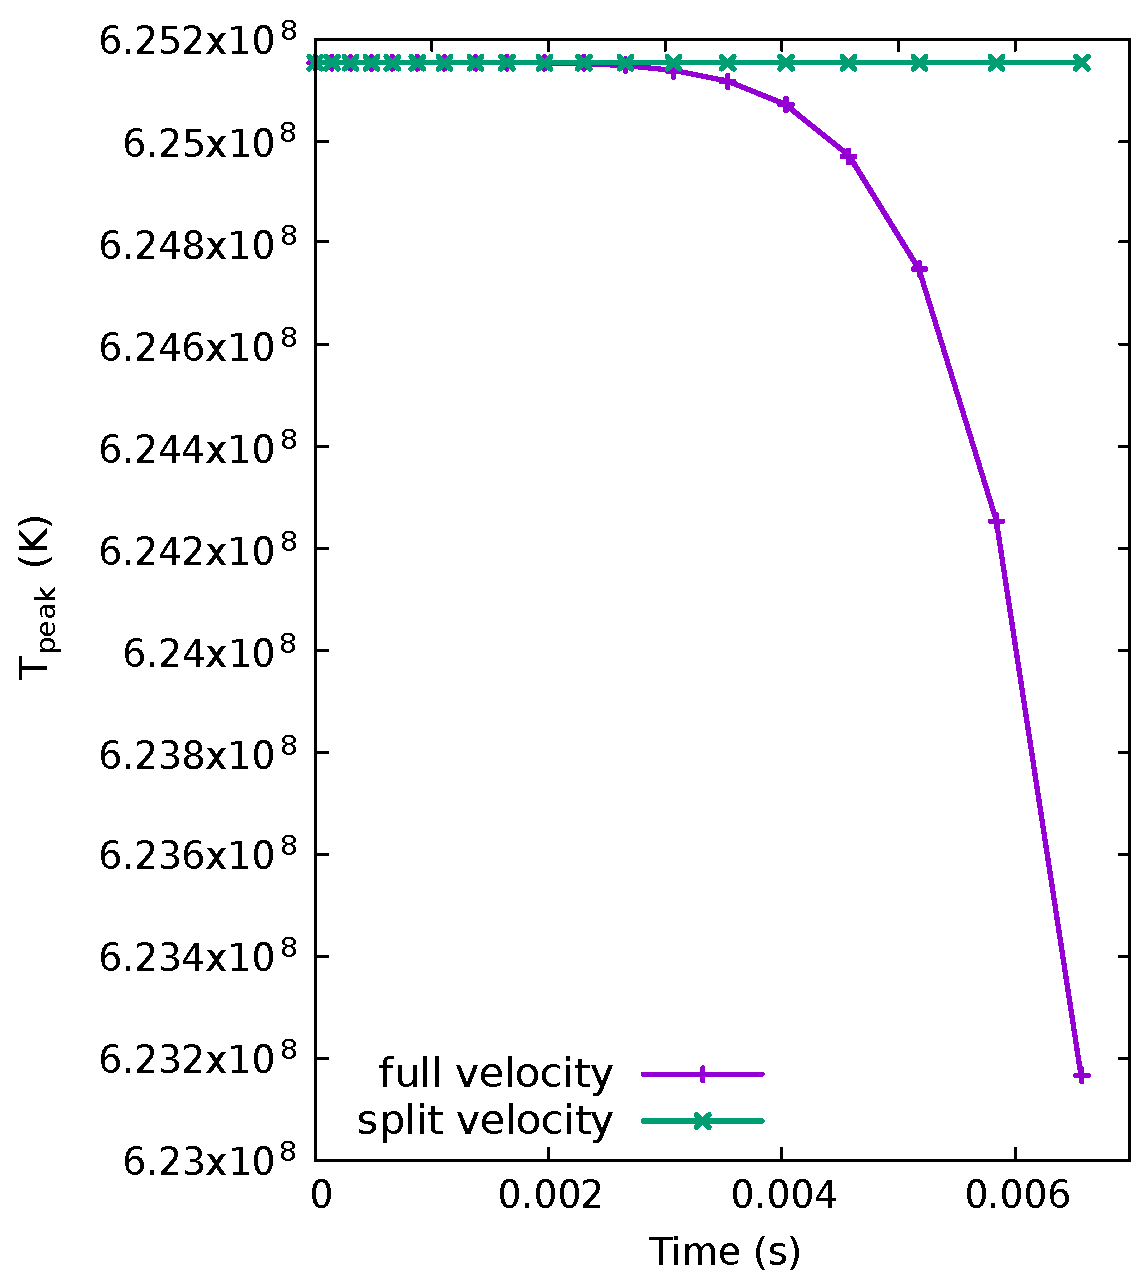
\includegraphics[width=3.0in]{./figs/wdconvect_256_splitU} } & \multicolumn{1}{c}{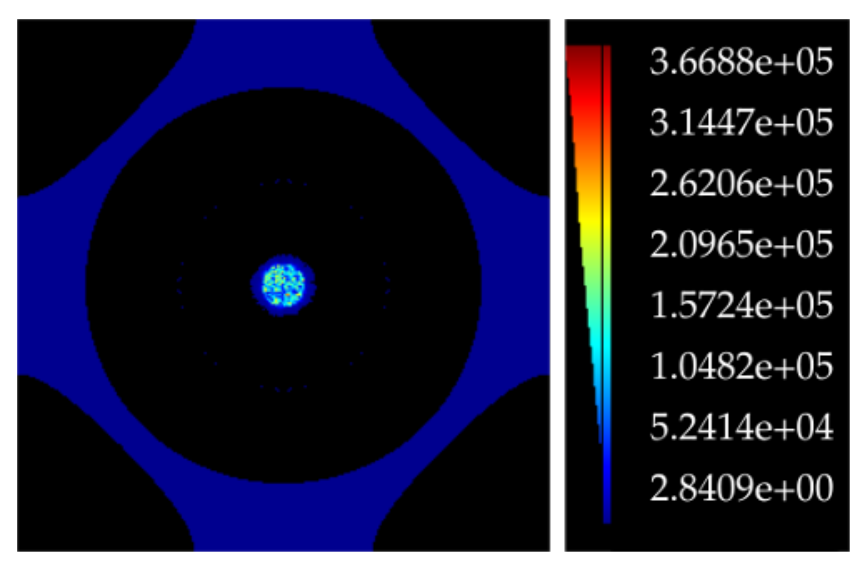
\includegraphics[width=2.35in]{./figs/magvel_full_XY}} \\
& \multicolumn{1}{c}{\begin{footnotesize} (a) $|\mathbf{U}|$, solved using $\mathbf{U}$ \end{footnotesize}} \\[1.em]
& \multicolumn{1}{c}{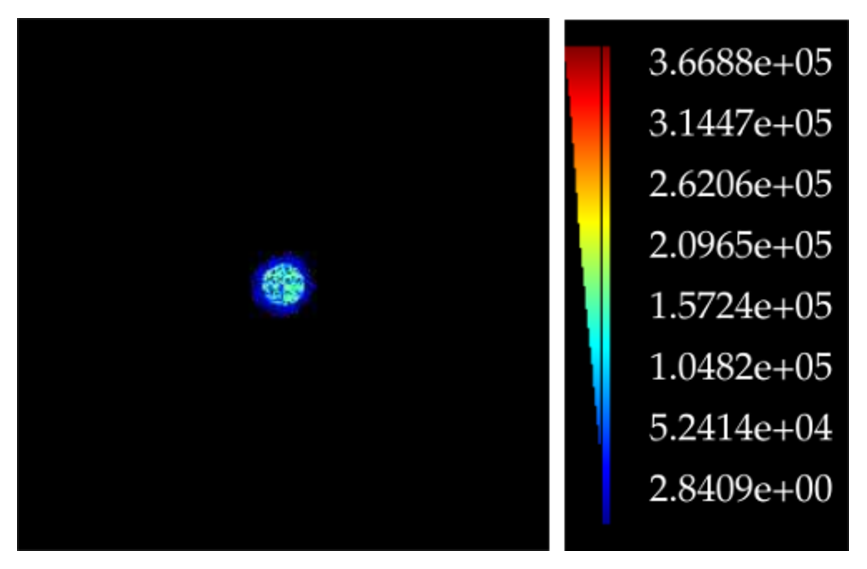
\includegraphics[width=2.35in]{./figs/magvel_split_XY}} \\ 
& \multicolumn{1}{c}{\begin{footnotesize} (b) $|\mathbf{U}|$, solved using $w_0 + \tilde{\mathbf{U}}$ \end{footnotesize}} \\
\end{tabular}
\caption{\label{fig:wdconvect_splitU} (Left) Peak temperature, $T_{\text{peak}}$ in a white dwarf at resolution of $256^3$ 
         during initial transition. (Right) Velocity magnitude solved using the full velocity $\mathbf{U}$ in projection step 
         results in large values outside the density cutoff region that is not seen with using the split velocities.}
\end{center}
\end{figure}
%%%%%%%%%%%%%%%%%%%%%%%%%%%%%

\section{Old Notes (not for inclusion in paper)}

\subsection{Exact Base State Notes}

\subsubsection{Potential Problems}
\begin{enumerate}
\item How do we define \verb|r_edge_loc| for irregularly-spaced base states whose cell-centered values are defined at $r_m=\Delta x\sqrt{\frac{3}{4} + 2m}$?
\item We would stil need to approximate the values at edges when advecting the base states (i.e. $\rho_0^{\nph,\pred}$). This may affect the nice properties we would get with exact cell-centered base state values.
\item Excessive memory storage may be required (\verb|nr_irreg >> nr_fine|).
\end{enumerate}

\subsubsection{A Possible Solution}
We could choose to no longer advect the base states for both predictor and corrector steps. This would solve the problems with computing state values at cell edges. Instead, we propose to only update the base states $\rho_0$ and $p_0$ by computing the average of the full state values after advecting the full states. This would result in the following changes in the algorithm from Paper V:
%
\begin{enumerate}
\item Steps 4 and 8 will be greatly simplified, leading to a more efficient algorithm.
\item \sout{There is no longer a need for $w_0$, so we can use the full velocity $\Ub$ instead of $\Ubt$. As a consequence, $\eta$ does not need to be computed. This has the added advantage of saving some memory storage by removing many of the terms needed when we decided to split terms into its base state and perturbation state in our previous implementation.} We split the velocity for the projection to handle the cutoff.
\item By placing the base states exactly at cell-centers, we eliminate interpolation errors and simplify the existing code.
\end{enumerate}
%

\subsection{$\eta_\rho$ Notes}
After {\bf Step 8D}, we define a radial cell-centered $\etarho^{\nph}$.

\begin{description}
\item For planar geometry, $\etarho = \overline{\rho'(\Ub\cdot\eb_r)}$,
\begin{equation}
 \etarho^{\nph} =  {\rm {\bf Average}} \sum_k \left[ \left(\uadvtwo \cdot \eb_r \right) (\rho X_k)^{\nph,\pred} \right]
\end{equation}
\item For spherical geometry, first construct 
$\etarho^{{\rm cart},\nph} = [\rho'(\Ub\cdot\eb_r)]^{\nph}$ on Cartesian cell centers using:
\begin{equation}
\etarho^{{\rm cart},\nph} = \left[\left(\frac{\rho^{(1)}+\rho^{(2)}}{2}\right)-\left(\frac{\rho_0^n+\rho_0^{n+1}}{2}\right)\right] \cdot \left( \uadvtwo \cdot \eb_r \right).
\end{equation}
Then,
\begin{equation}
\etarho^{\nph,\star} = {\rm {\bf Average}}\left(\etarho^{{\rm cart},\nph}\right).
\end{equation}
\end{description}

\subsection{Computing $w_0$ For Spherical Problems}
Recall that we want to solve
\begin{equation}
\frac{1}{r^2}\frac{\partial}{\partial r}(r^2 w_0) = \Sbar - \frac{1}{\gammaonebar p_0}\left(\frac{\partial p_0}{\partial t} + w_0\frac{\partial p_0}{\partial r}\right)
\end{equation}
First, note that $\partial p_0/\partial r = -\rho_0 g$.
The key observation here is that we can compute $\partial p_0/\partial t$ directly instead of making complicated substitutions involving $\eta_\rho$ to eliminate it.
Let's discretize this as follows:
\begin{equation}
\frac{1}{r_j^2}\left[\frac{\left(r^2 w_0\right)_{j+\myhalf} - \left(r^2 w_0\right)_{j-\myhalf}}{\Delta r}\right] = 
\Sbar_j - \frac{1}{\left(\gammaonebar p_0\right)_j}\left[\left(\frac{\partial p_0}{\partial t}\right)_j - \left(\frac{w_{0,j-\myhalf}+w_{0,j+\myhalf}}{2}\right)(\rho_0 g)_j\right]
\end{equation}
Rearranging this to solve for $w_{0,j+\myhalf}$ gives us an explicit update:
\begin{equation}
\left[\frac{r_{j+\myhalf}^2}{r_j^2\Delta r} - \frac{(\rho_0 g)_j}{2\left(\gammaonebar p_0\right)_j}\right] w_{0,j+\myhalf} =
\left[\frac{r_{j-\myhalf}^2}{r_j^2\Delta r} + \frac{(\rho_0 g)_j}{2\left(\gammaonebar p_0\right)_j}\right] w_{0,j-\myhalf}
+ \Sbar_j - \frac{1}{\left(\gammaonebar p_0\right)_j}\left(\frac{\partial p_0}{\partial t}\right)_j
\end{equation}
As before, once $\rho_0$ falls below $\rho_{\rm cutoff}$, we hold $r^2 w_0$ constant.\\ \\
The interface to the routine in the algorithm description is
{\bf Make $\mathbf{w_0}$}$[\rho_0,p_0,\partial p_0/\partial t,\gammaonebar,\Sbar] \rightarrow [w_0]$

\subsection{TODO List}

TODO list:
\begin{itemize}
\item Weak scaling tests of original algorithm, comparing MAESTRO to MAESTROeX.  Use cori knl, 4 MPI per node, 16 threads per MPI
\item Run at effective $512^3$ resolution (maybe to ignition?... need to see how max T trends go) (1) classic MAESTRO, (2) MAESTROeX with original algorithm, (3) MAESTROeX with new temporal integrator, (4) MAESTROeX with new temporal integrator and irregular dr, (5) MAESTROeX with original algorithm and 3-levels of AMR, (6) MAESTROeX with new temporal integrator and 3 levels of AMR.
\item (perhaps) a demonstration of what goes wrong when you don't split the velocity dynamics in the projection
\end{itemize}



\bibliographystyle{aasjournal.bst}
\bibliography{references}

\end{document}
